\chapter{Test}

\label{ch:test}

	\section{Servo test}

	\hspace{15pt}Our first plan was to test all of the servos and the robot's possibilities. We reached that because we implemented a test software which can communicate with the laptop on serial. 
	
	
	The program firstly set all the servos to center and after that relax all of them.The software's input is the servo number and the requested position (from 0 to 1023) and after that the robot's servo motor set that parameter to the selected servo. With this we could test all the servos. The basic code is the following:
	
	\lstinputlisting[language={C++}]{implementation/basic_test/basic_test.ino}
	
	\section{Position tests}
		
		\subsection{Position 1 test}
		
			\hspace{15pt}In the first test case we would like to check if the robotic arm can reach a vertically stretched position with a closed pincher tool.

			We need the following inputs for this action:

			\begin{enumerate}
				\item $x = 0$ \\
				\item $y = 0$ \\
				\item $z = 385$ \\
				\item $\phi = 0°$ \\
				\item $pincher = closed$ \\
			\end{enumerate}

			Why is the value of z exactly 385?. We have an easy answer for it. Please see the constant values about the robotic arm’s sizes, and you can easily calculate that it is the fully stretched length of the device in millimeters.
		
			\begin{figure}[H]
				\centering
				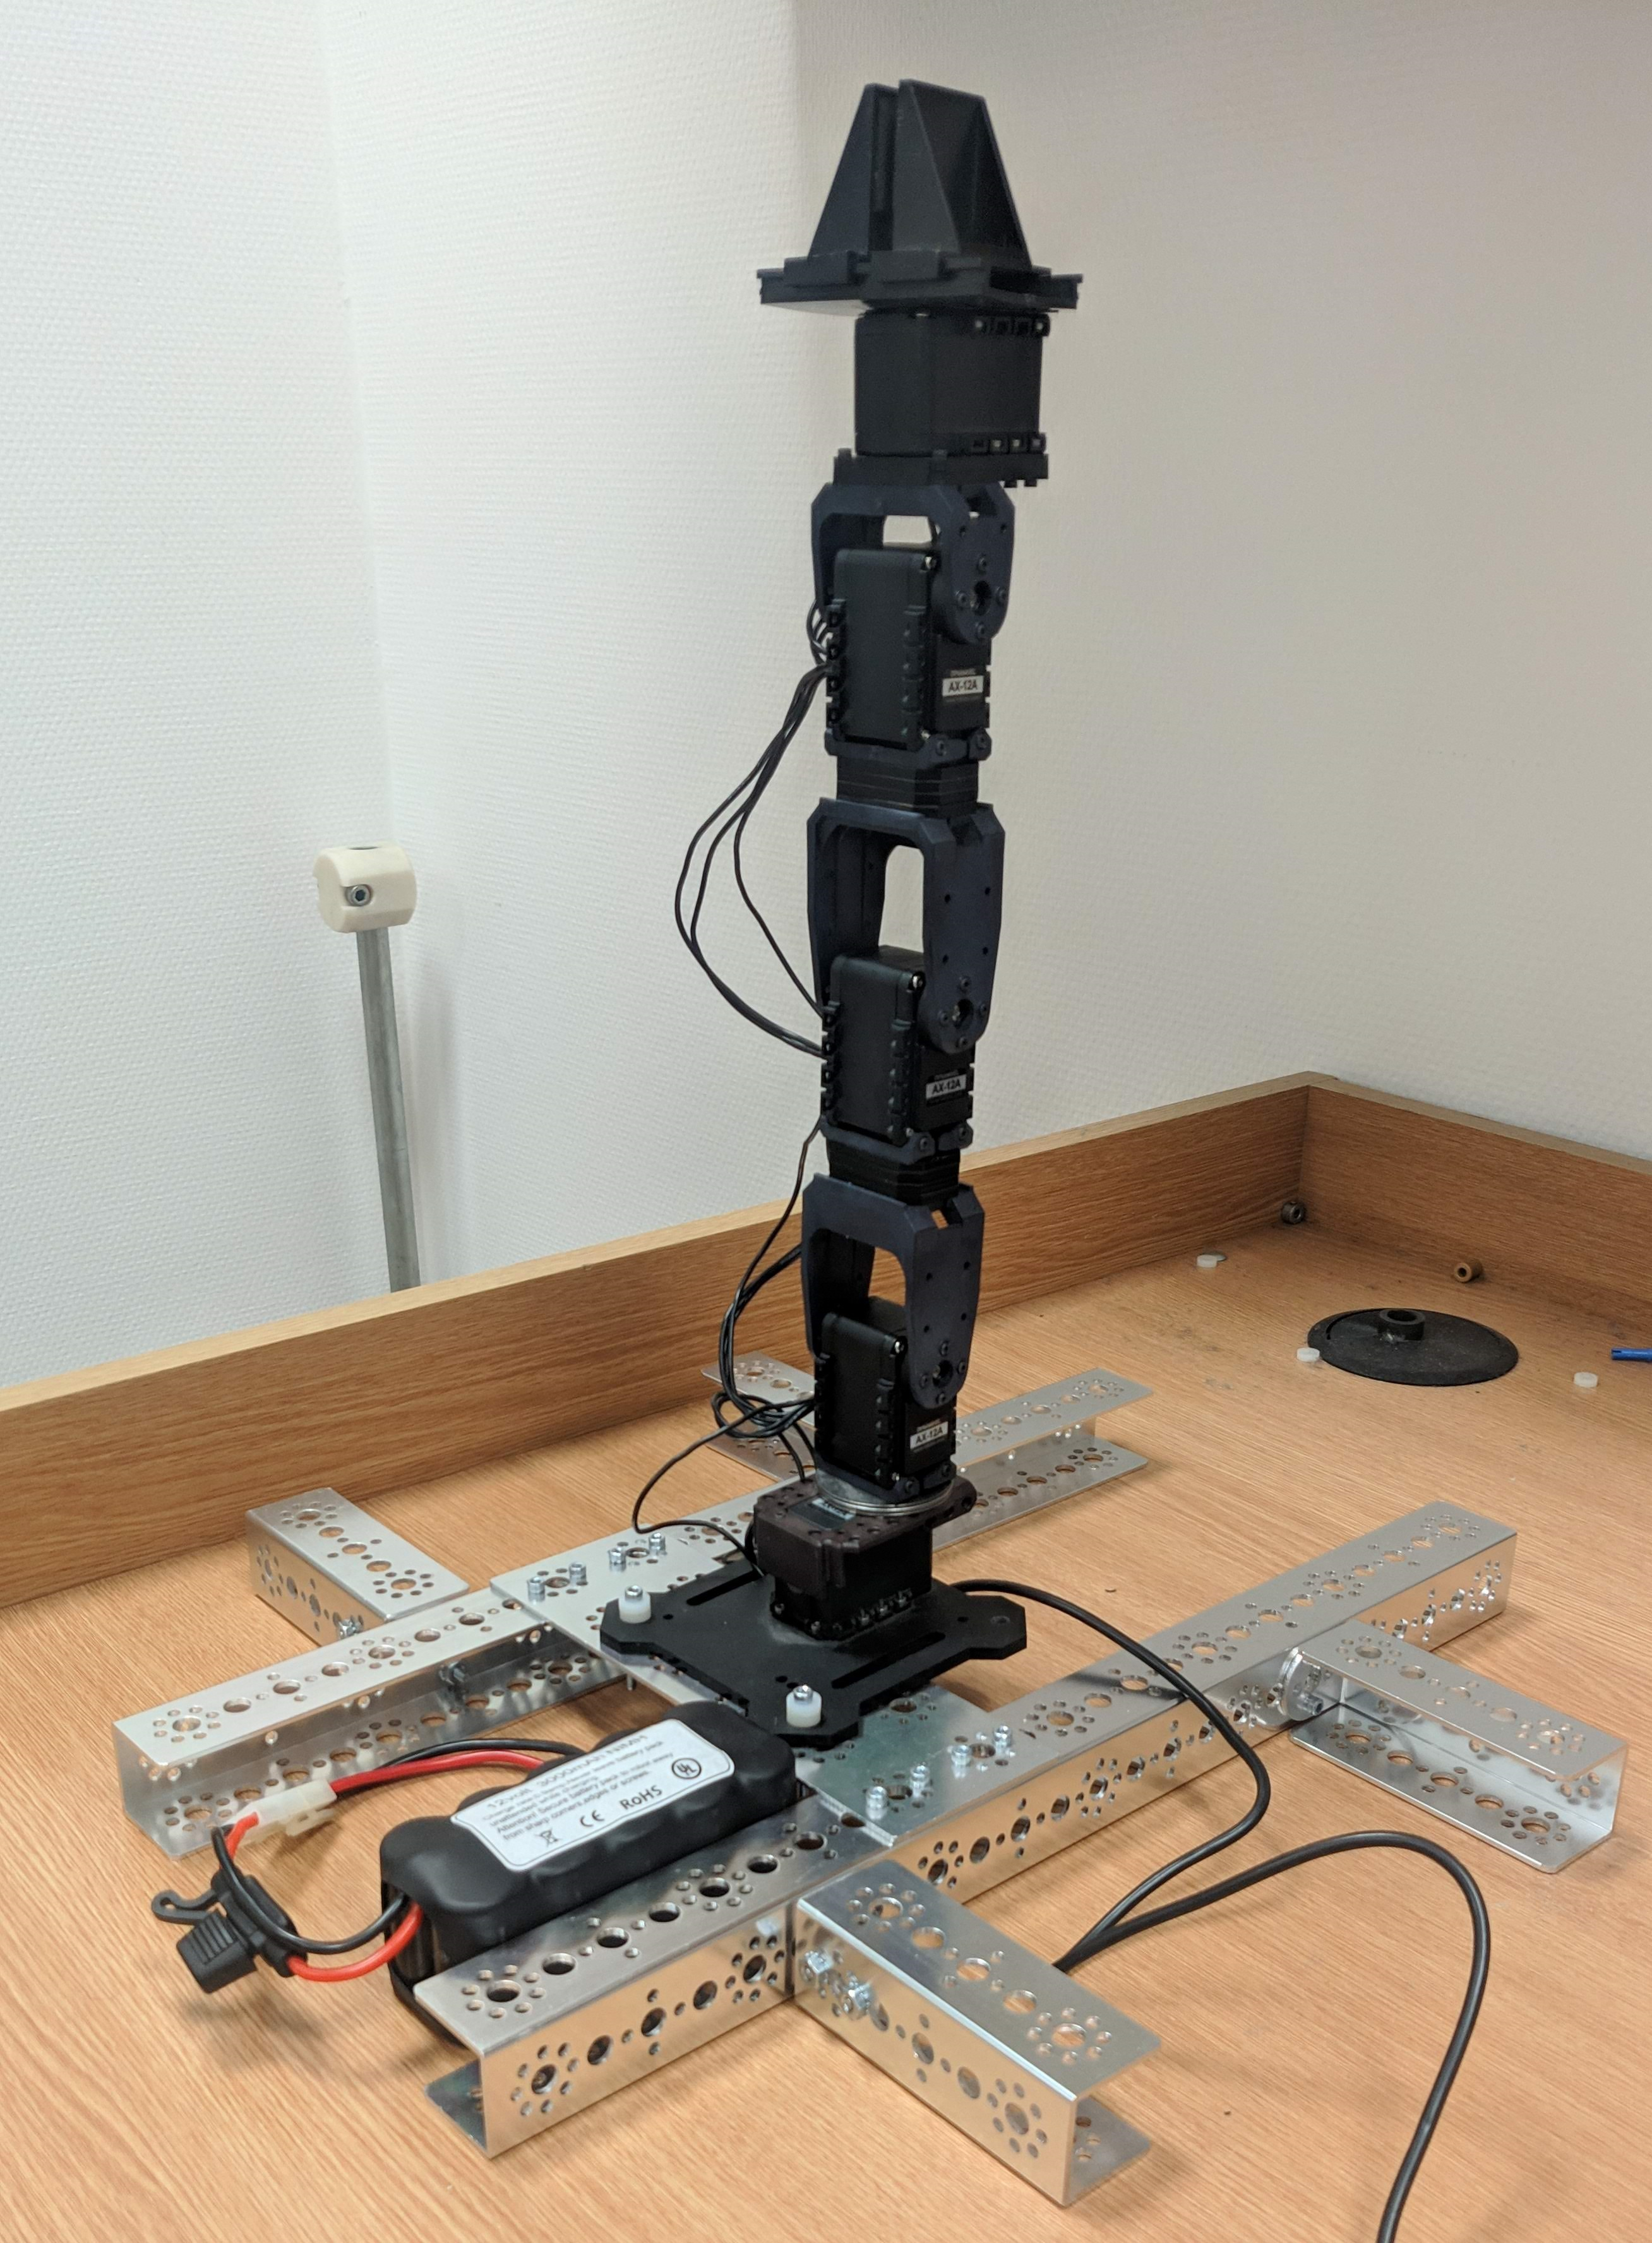
\includegraphics[scale=0.11]{./images/test_center}
				\caption{Center test (0,0,385) 0°}
			\end{figure}
			
			Output:
			
			\begin{verbatim}
				###########################
				Serial Communication Established.
				###########################
				Set all servo motor to center (512).
				###########################
				X position: 0
				###########################
				Y position: 0
				###########################
				Z position: 385
				###########################
				Phi degree: 0°
				###########################
				Pincher (0/1): 0
				###########################
				Position: (0,0,385) 0 rad | Pincher: 0
				###########################
				Teta1: 0
				Teta2: 0
				Teta3: 0
				Teta4: 0
				Pos1: 512
				Pos2: 512
				Pos3: 512
				Pos4: 512
				Pincher pos: 0
				Send a random character if you want to set another position
			\end{verbatim}
			
		\subsection{Position 2 test}
		
			\hspace{15pt}In the second test case we simulate a real situation where the robotic arm has to hold an object quite high in its own coordinate system, and this test case shows the strength of the device holding an object while the last joint is turned 90 degrees.

			Here are the input values for this case:

			\begin{enumerate}
				\item $x = 0$ \\
				\item $y = 101$ \\
				\item $z = 284$ \\
				\item $\phi = 90°$ \\
				\item $pincher = closed$ \\
			\end{enumerate}
		
			\begin{figure}[H]
				\centering
				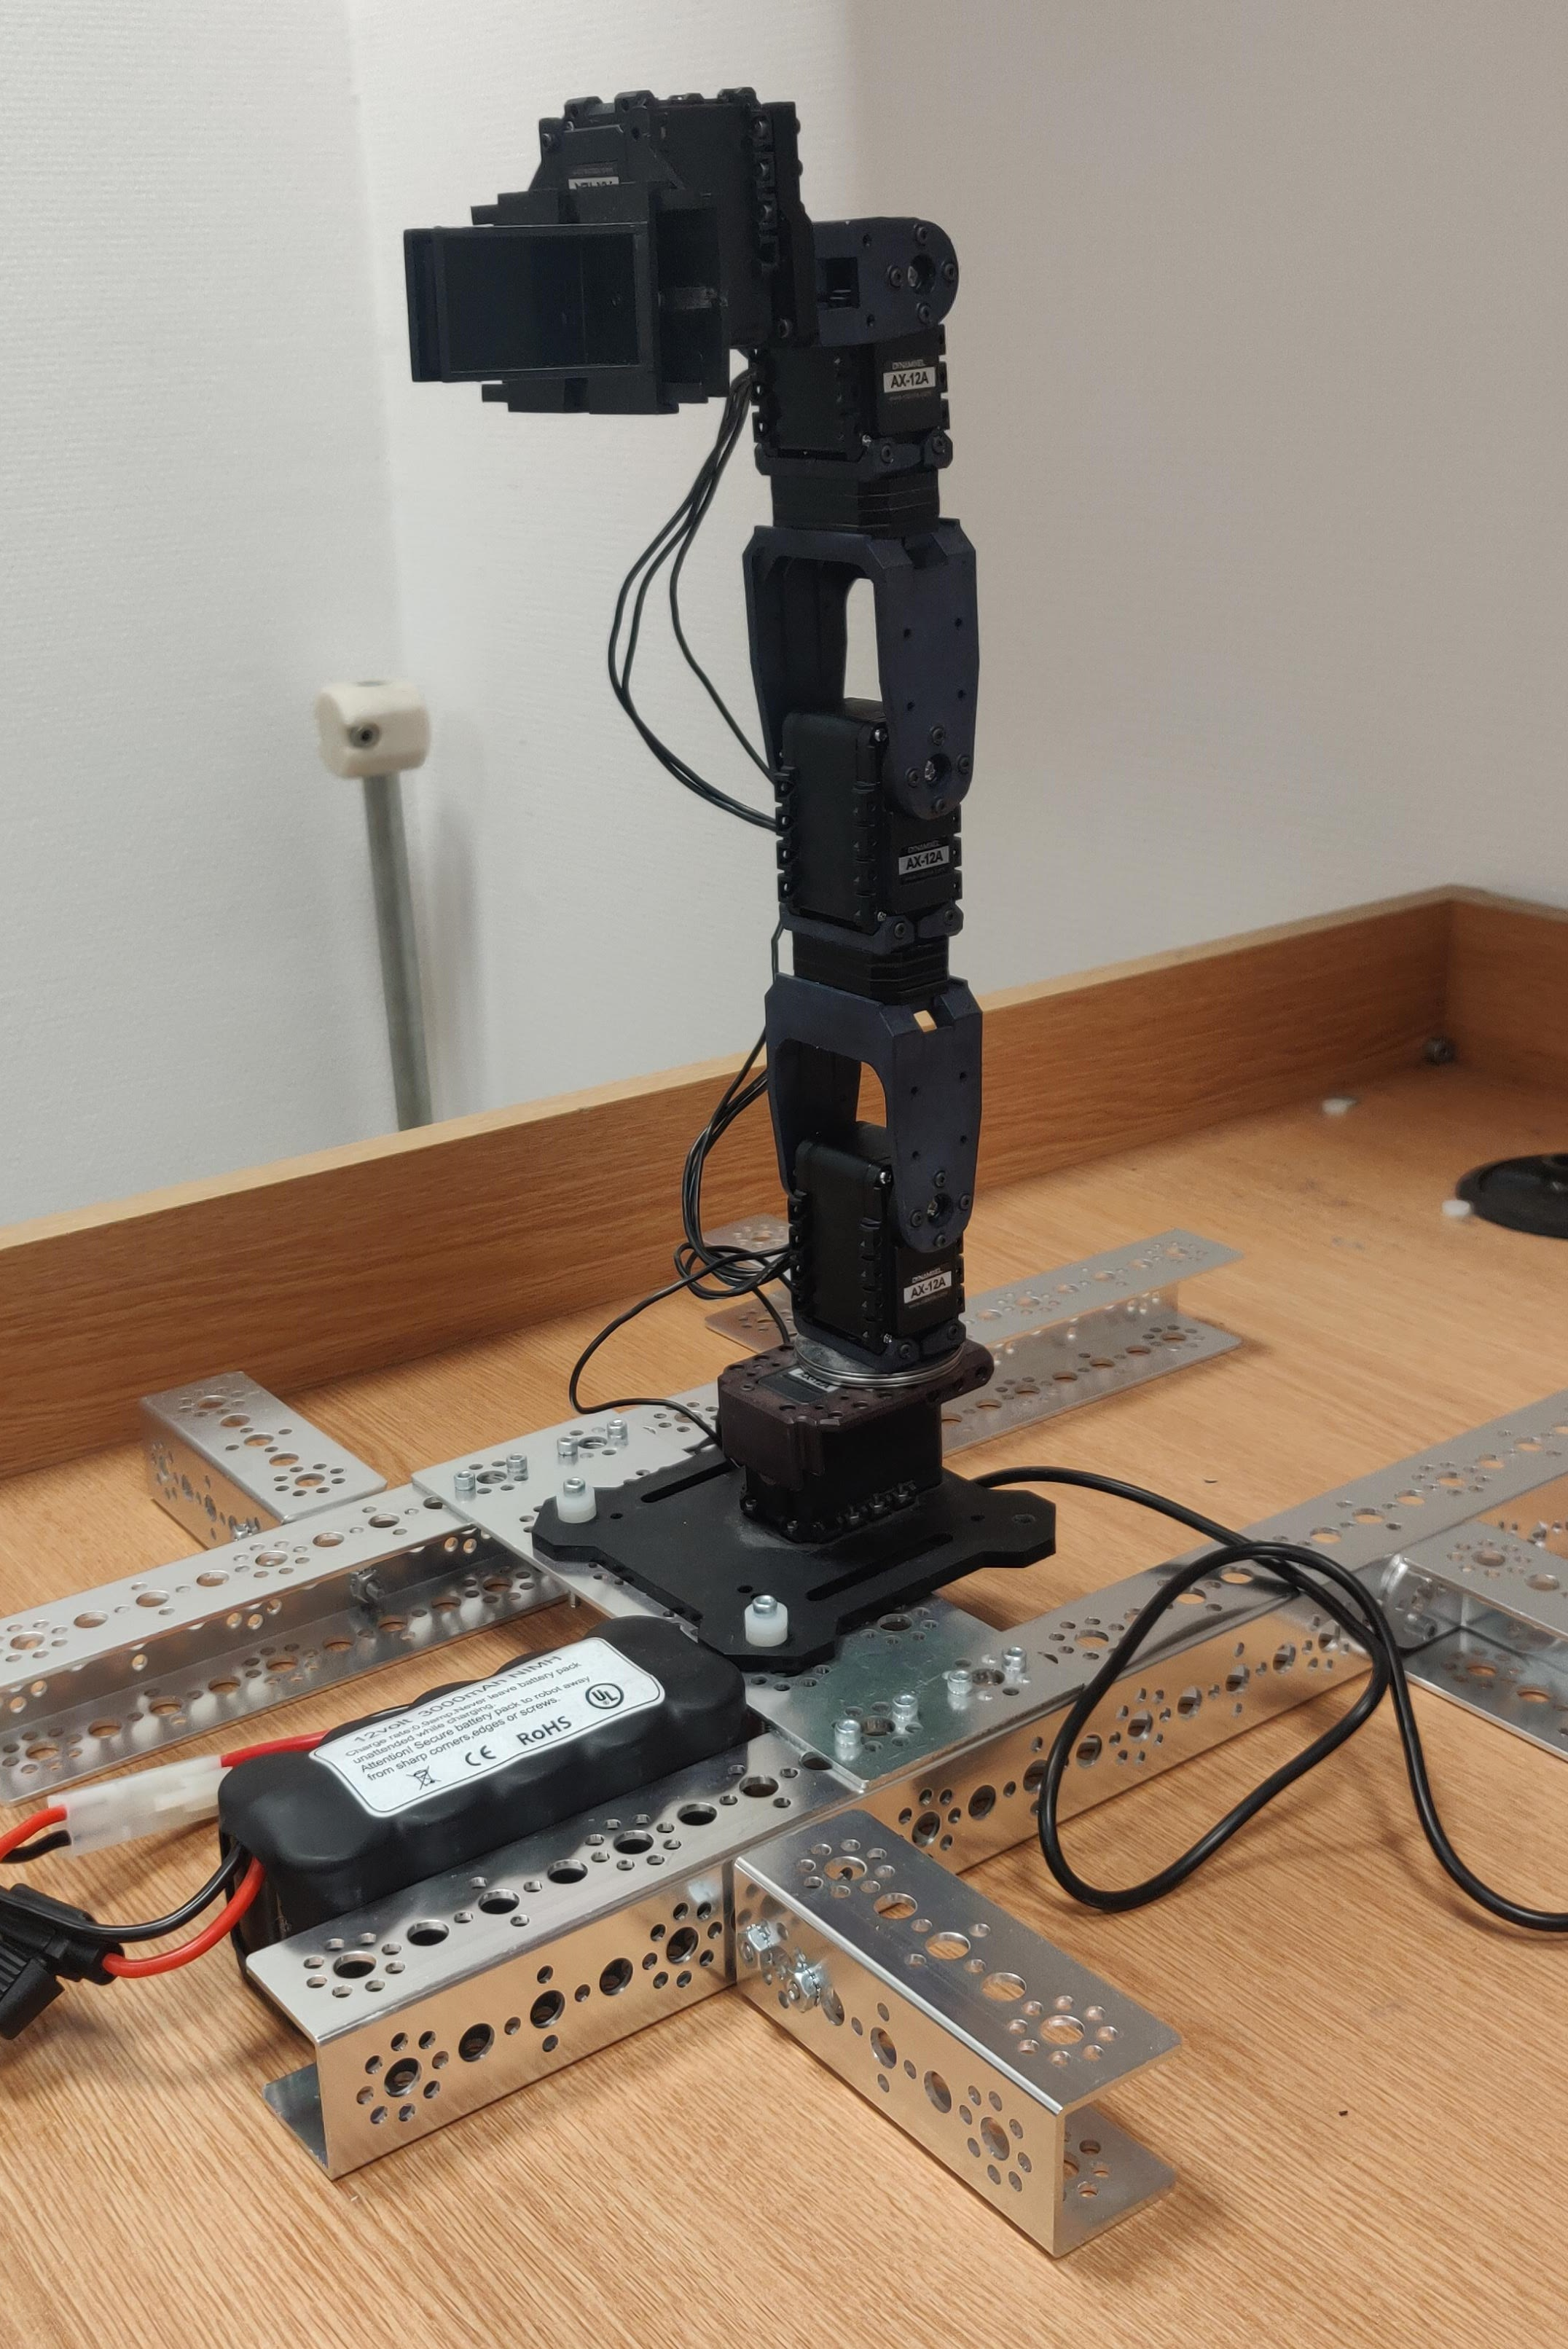
\includegraphics[scale=0.11]{./images/test_2}
				\caption{Position test (0,101,284) 90°}
			\end{figure}
			
			Output: 
			
			\begin{verbatim}
				###########################
				Serial Communication Established.
				###########################
				Set all servo motor to center (512).
				###########################
				X position: 0
				###########################
				Y position: 101
				###########################
				Z position: 284
				###########################
				Phi degree: 3.14
				###########################
				Pincher (0/1): 0
				###########################
				Position: (0,101,284) 1.57 rad | Pincher: 0
				###########################
				Teta1: 0
				Teta2: 0
				Teta3: 0
				Teta4: 1.57
				Pos1: 512
				Pos2: 512
				Pos3: 512
				Pos4: 768
				Pincher pos: 0
				Send a random character if you want to set another position
			\end{verbatim}
			
		\subsection{Position 3 test}
		
			\hspace{15pt}In this case we involve the second joint too and test its function, in a simple example. If you see the test cases as a process you can notice that we are simulating an object’s slow placing on the ground. If we execute the test cases in reverse order then we can test the lifting of an object too. 
			
			We use the following input data here:
		
			\begin{enumerate}
				\item $x = 0$ \\
				\item $y = 101$ \\
				\item $z = 82$ \\
				\item $\phi = 180°$ \\
				\item $pincher = closed$ \\
			\end{enumerate}
		
			\begin{figure}[H]
				\centering
				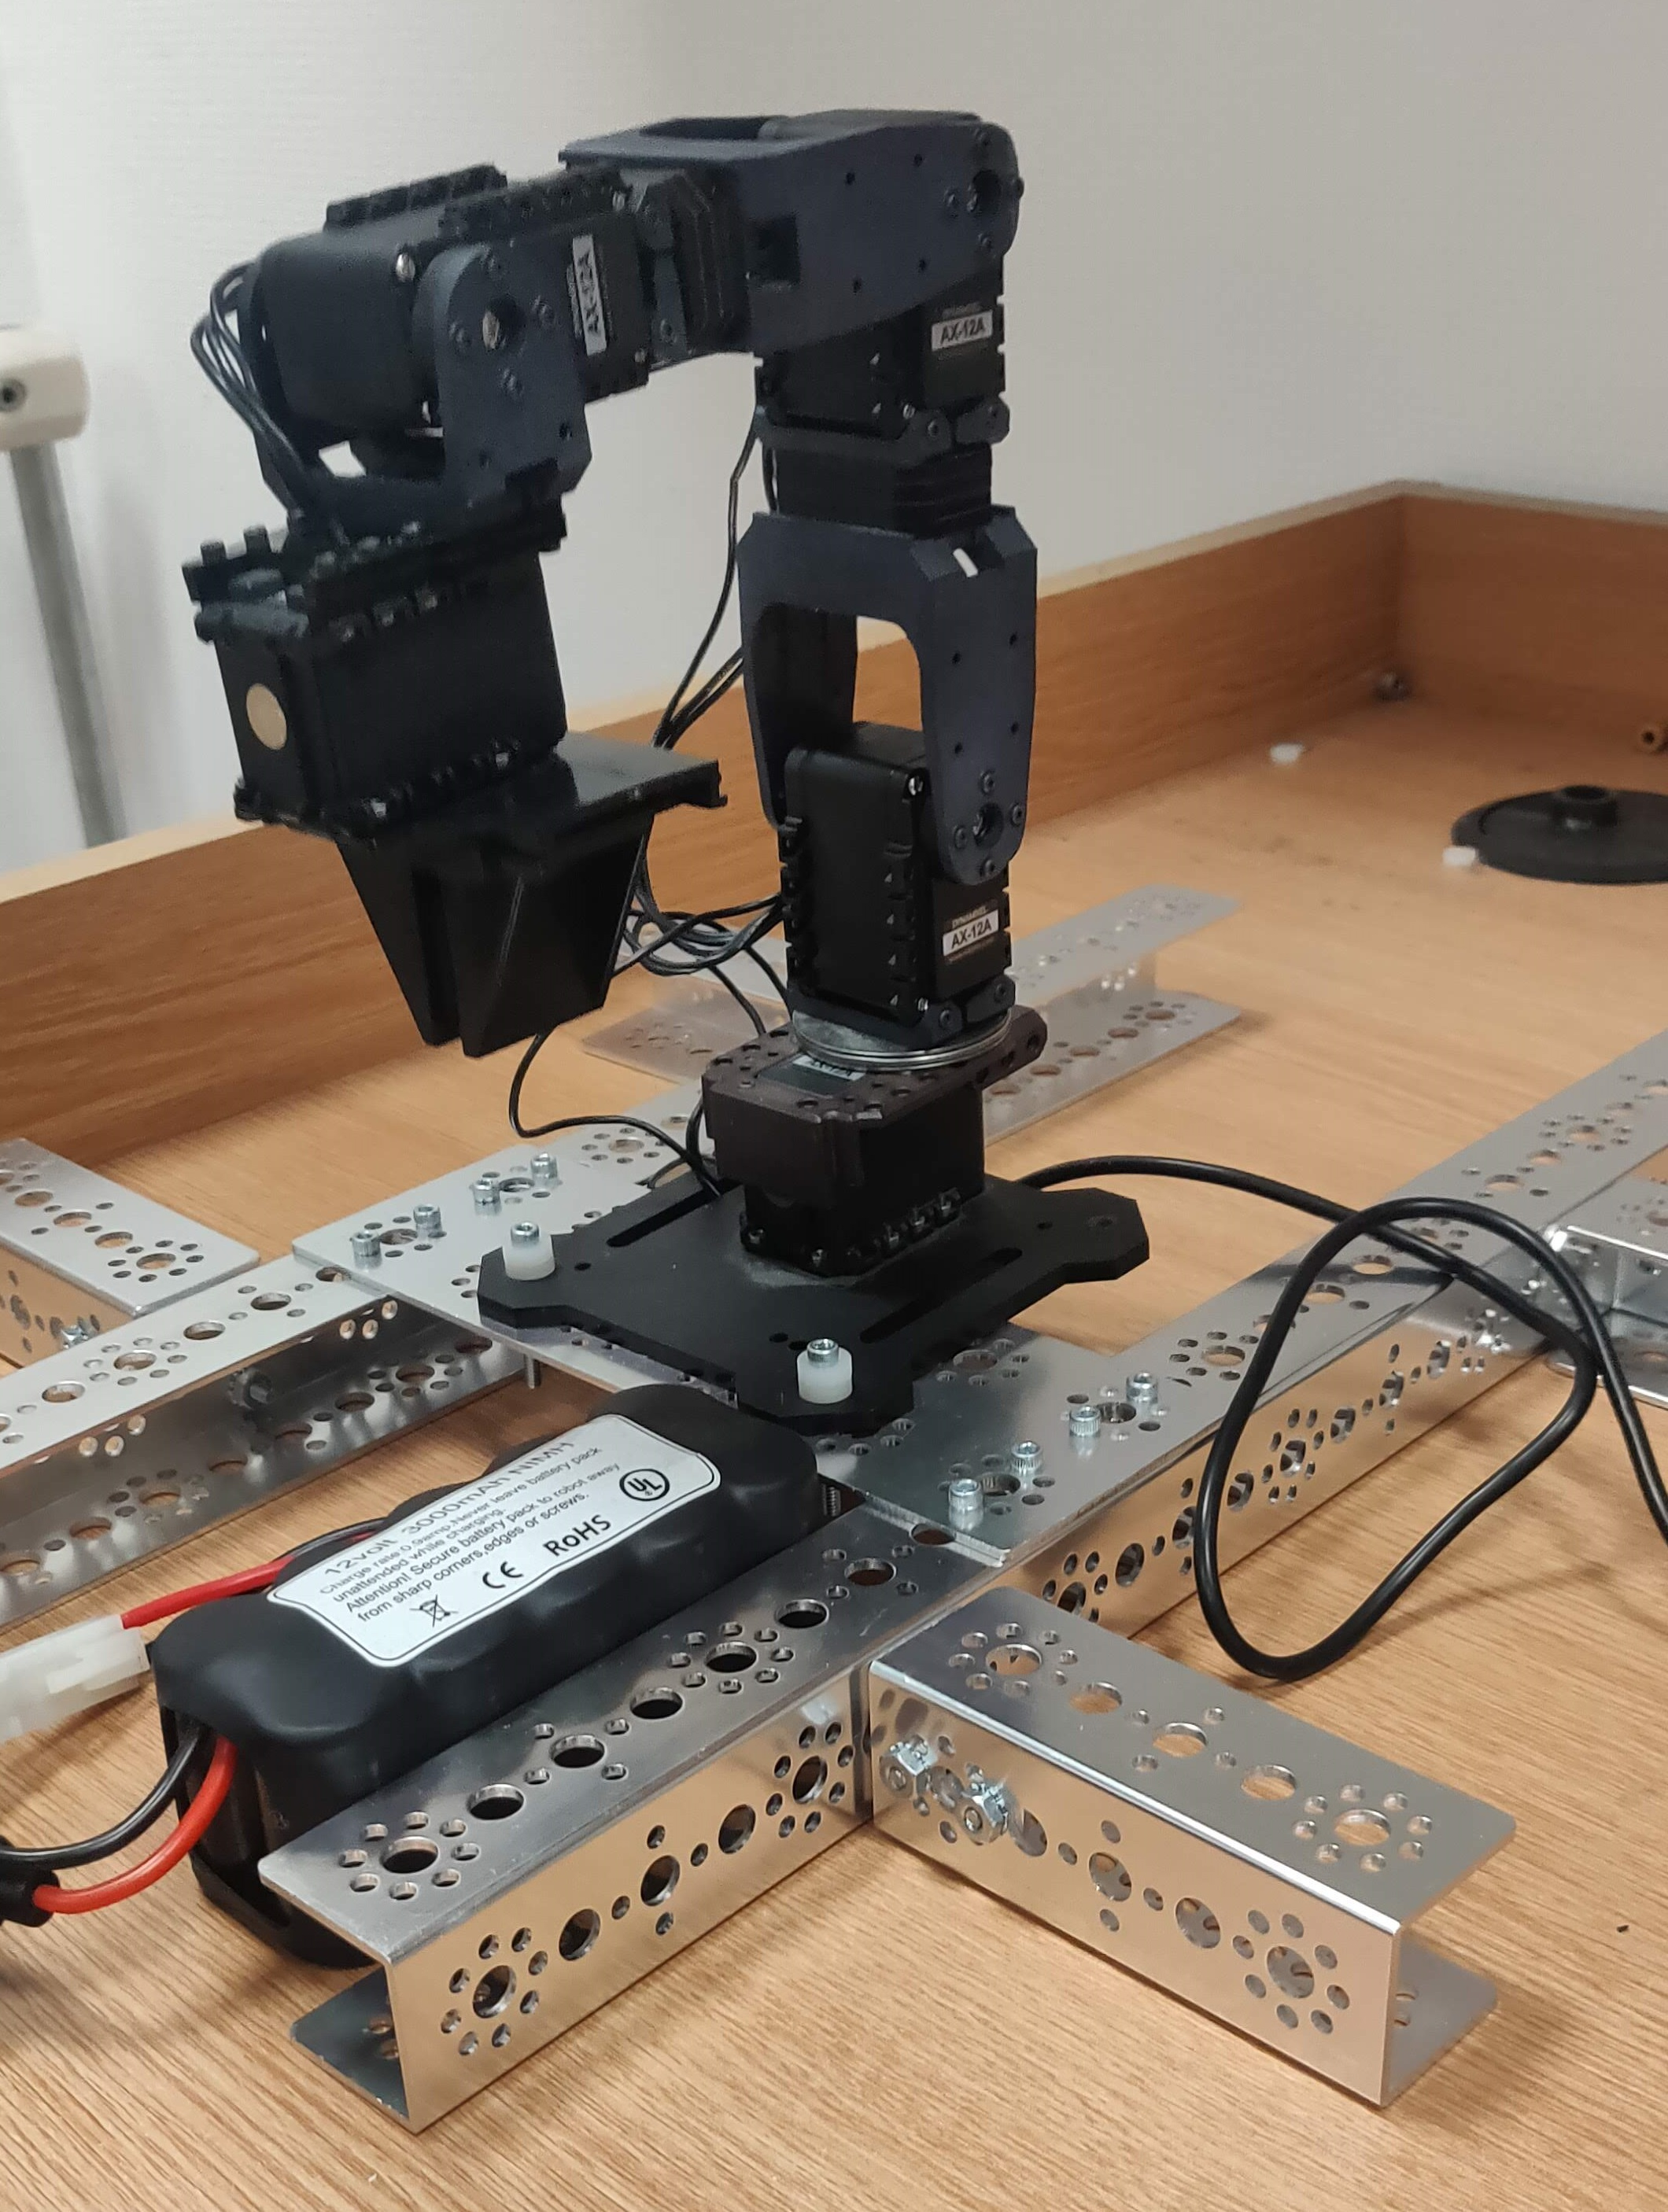
\includegraphics[scale=0.11]{./images/test_3}
				\caption{Position test (0,101,82) 180°}
			\end{figure}
			
			Output: 
			
			\begin{verbatim}
				###########################
				Serial Communication Established.
				###########################
				Set all servo motor to center (512).
				###########################
				X position: 0
				###########################
				Y position: 101
				###########################
				Z position: 284
				###########################
				Phi degree: 180°
				###########################
				Pincher (0/1): 0
				###########################
				Position: (0,101,82) 3.14 rad | Pincher: 0
				###########################
				Teta1: 0
				Teta2: 0
				Teta3: 1.57
				Teta4: 1.57
				Pos1: 512
				Pos2: 512
				Pos3: 768
				Pos4: 768
				Pincher pos: 0
				Send a random character if you want to set another position
			\end{verbatim}
			
		\subsection{Evaluation}
		
			\space{15pt}If all the basic test cases are passed we can judge our system as failure-free, and the robotic arm can hold and moved objects which are not heavier then specified in the pincher tool’s datasheet.